\subsection{Mosquitto Broker}\label{sw_mqtt-broker}
Als erste wichtige Erweiterung benötigen wir für unseren Home Assistant einen MQTT Broker. 
Da wir eine Supervised Version des Home Assistant auf unserem Pi vewenden, nutzen wir für die Installation den Supervisor Add-on Shop von Home Assistant (vgl. Abb.  \ref{fig:ha11}: \nameref{fig:ha11}).\\
\noindent Hier wählen wir den Mosquitto Broker zur Installation aus (vgl. Abb. \ref{fig:ha12}: \nameref{fig:ha12}). 
Um den Mosquitto Broker zu aktivieren, navigieren wir über den Menüpunkt ,,Einstellungen'' zum Punkt ,,Integrationen'' und suchen dort nach MQTT. 
Wir aktivieren die Verknüpfung von Home Assistant und Mosquitto Broker, indem wir die Schaltfläche ,,Suche aktivieren'' klicken.
Nach Durchführung dieser Schritte ist der Mosquitto Broker aktiv.
\begin{figure}[H]
    \begin{subfigure}{.5\linewidth}
        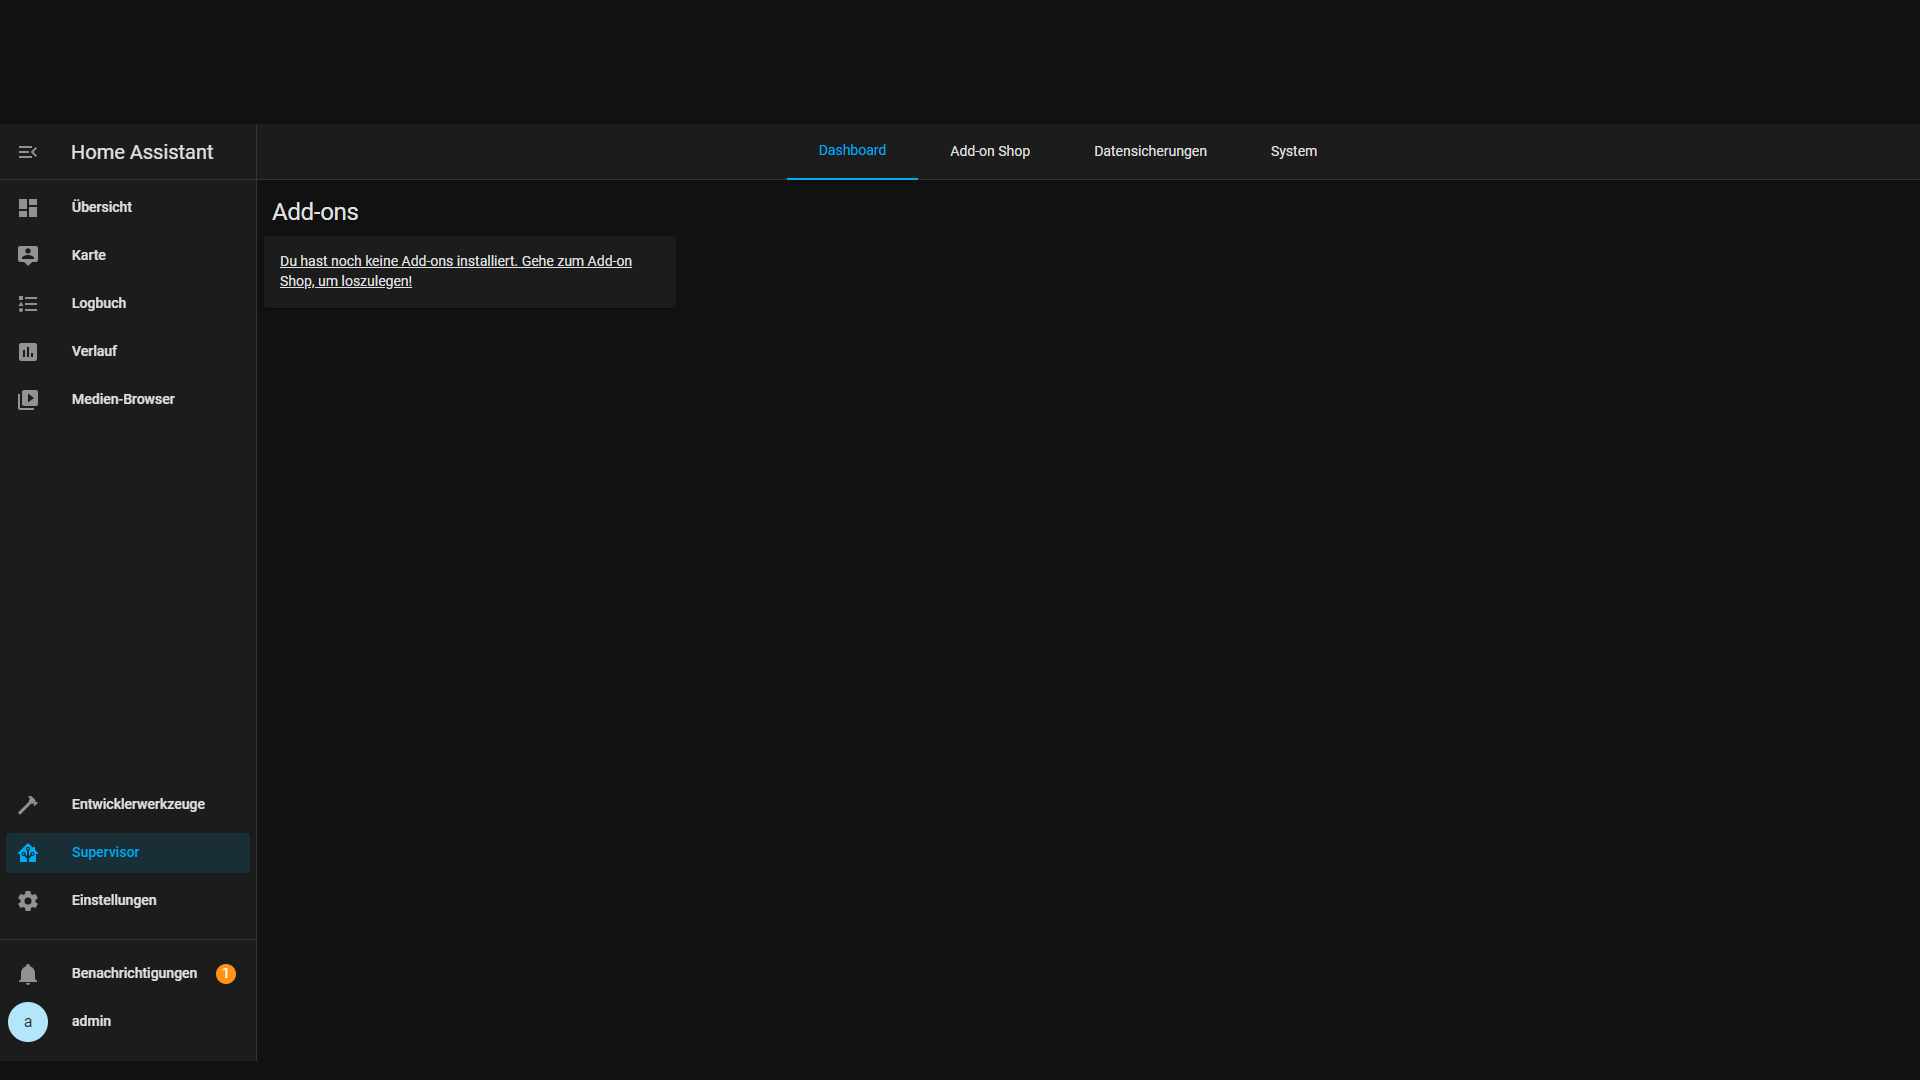
\includegraphics[width=1\textwidth]{img/HA6.png}
        \caption{Supervisor Dashboard}
        \label{fig:ha5}
    \end{subfigure}
    \begin{subfigure}{.5\linewidth}
        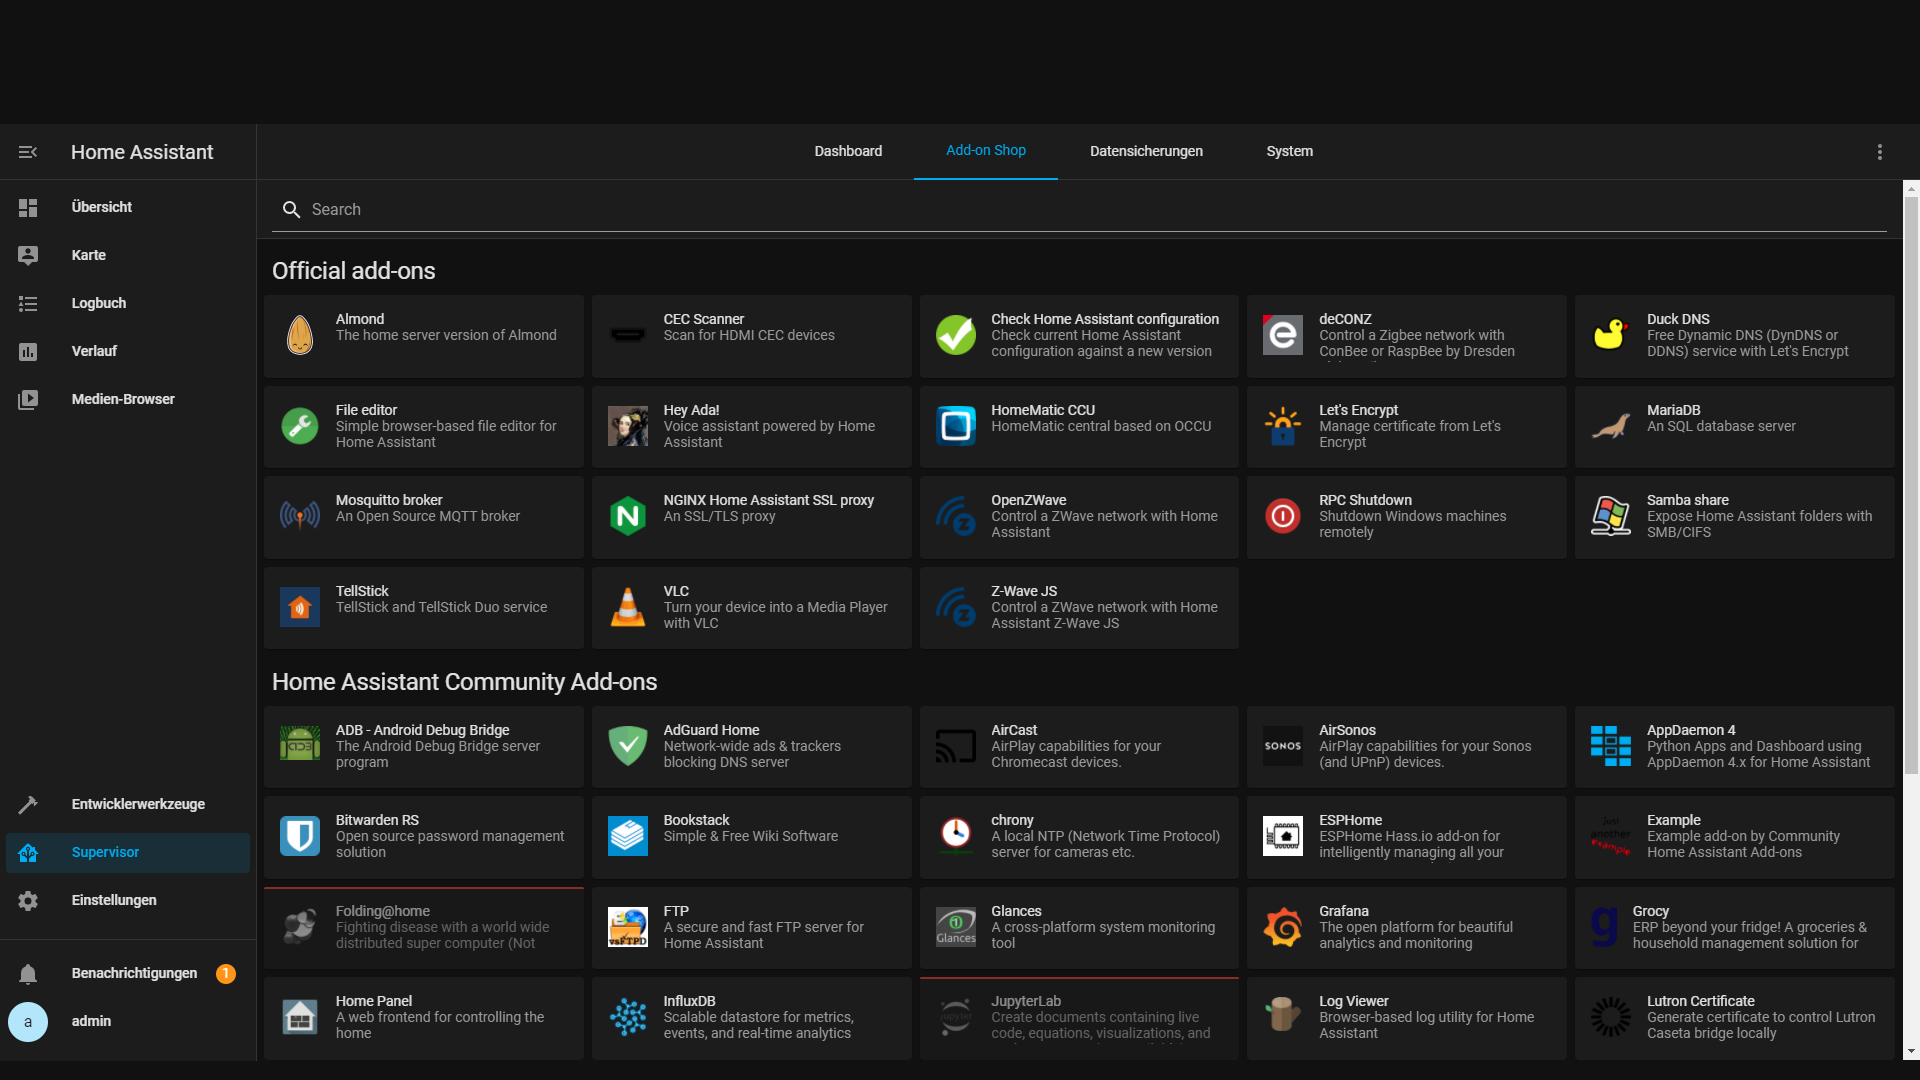
\includegraphics[width=1\textwidth]{img/HA7.png}
        \caption{Supervisor Add-on Shop}
        \label{fig:ha6}
    \end{subfigure}
    \begin{subfigure}{.5\linewidth}
        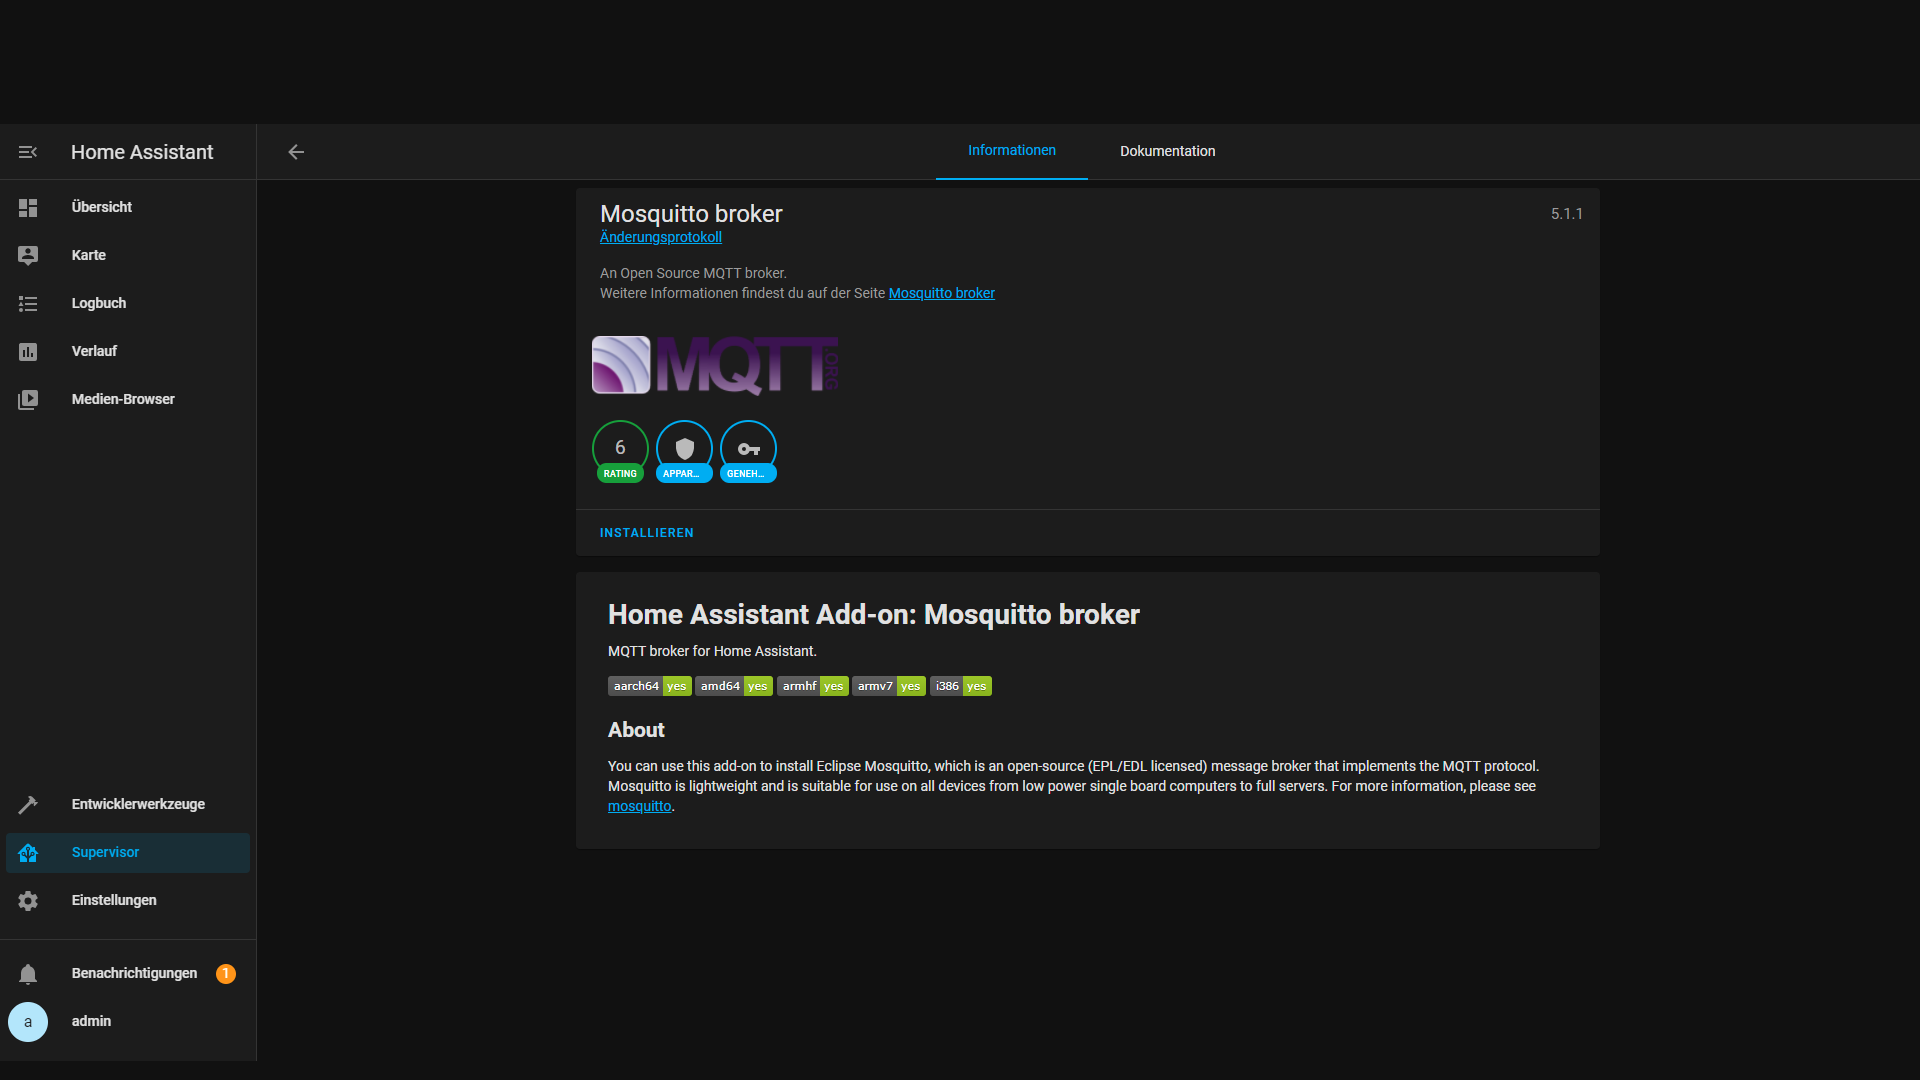
\includegraphics[width=1\textwidth]{img/HA8.png}
        \caption{MQTT add-on seite}
        \label{fig:ha7}
    \end{subfigure}
    \begin{subfigure}{.5\linewidth}
        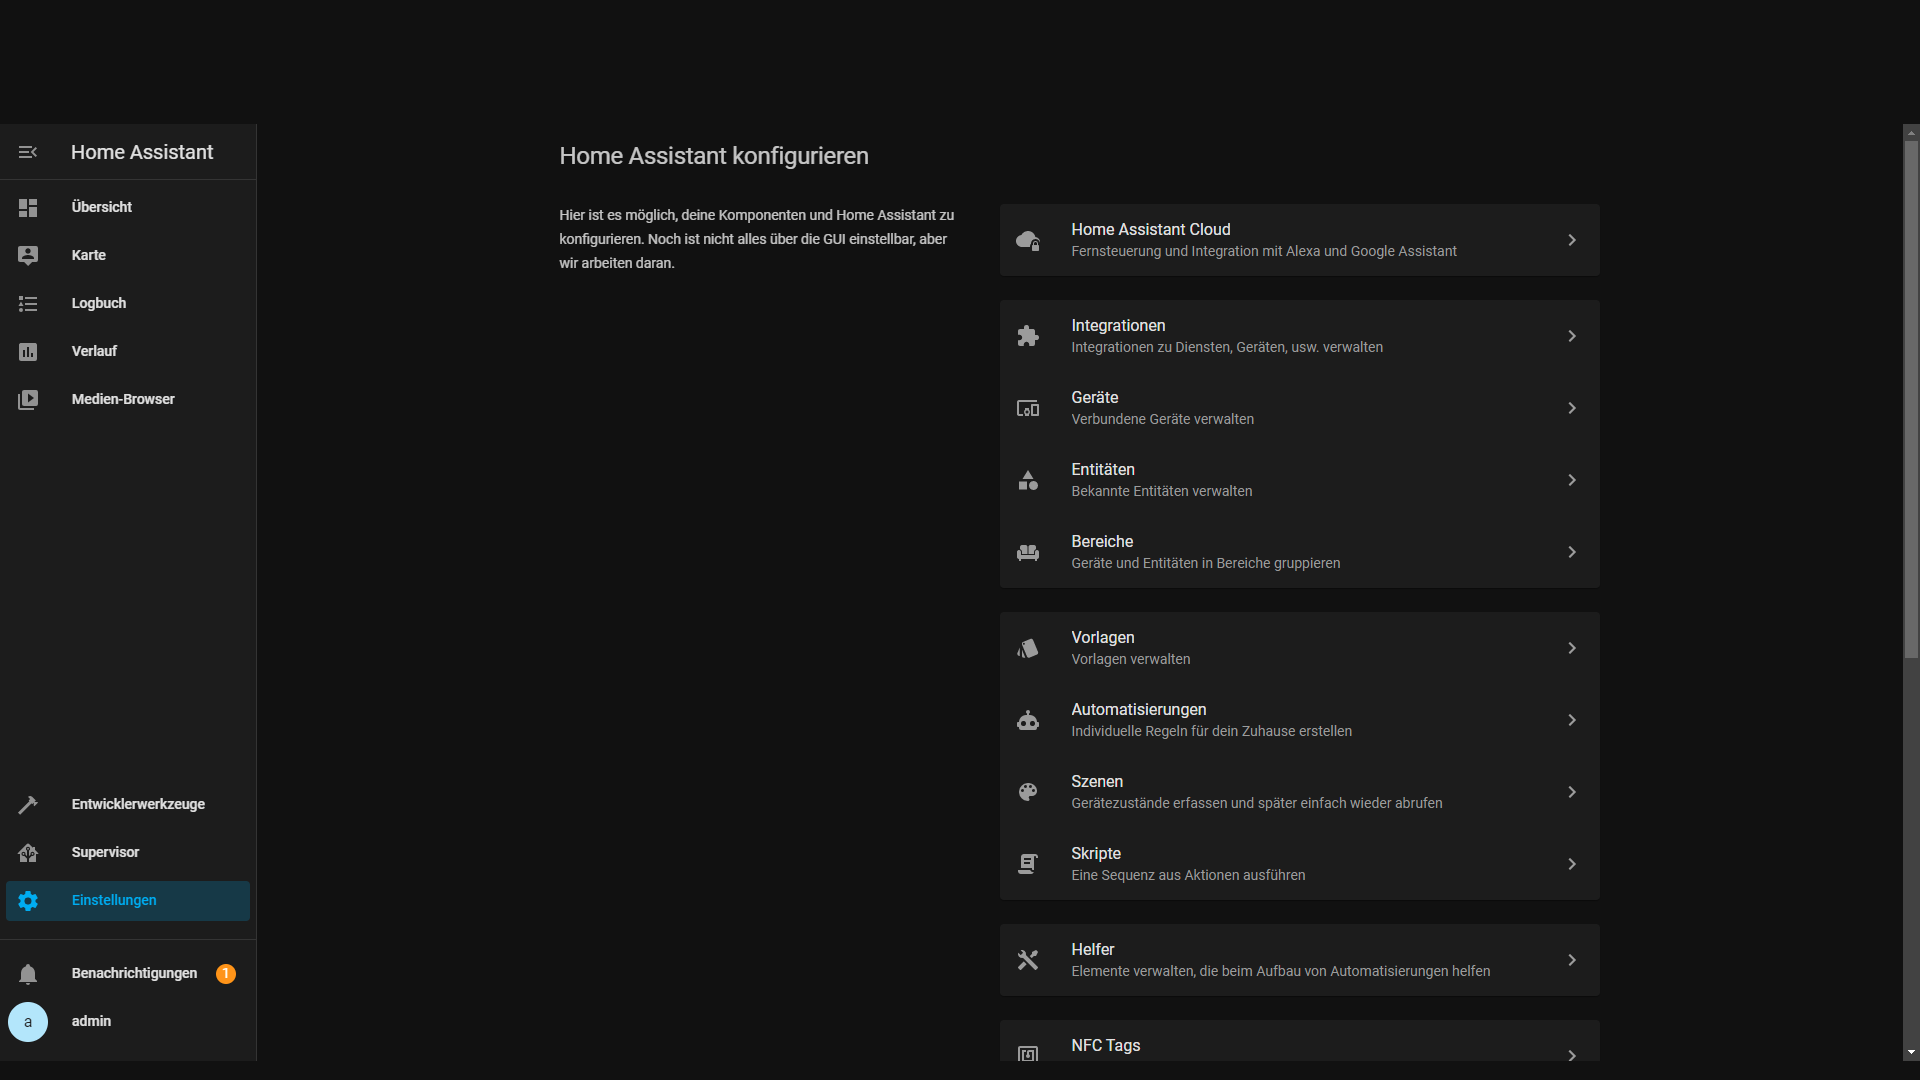
\includegraphics[width=1\textwidth]{img/HA9.png}
        \caption{Einstellungen}
        \label{fig:ha8}
    \end{subfigure}
    \begin{subfigure}{.5\linewidth}
        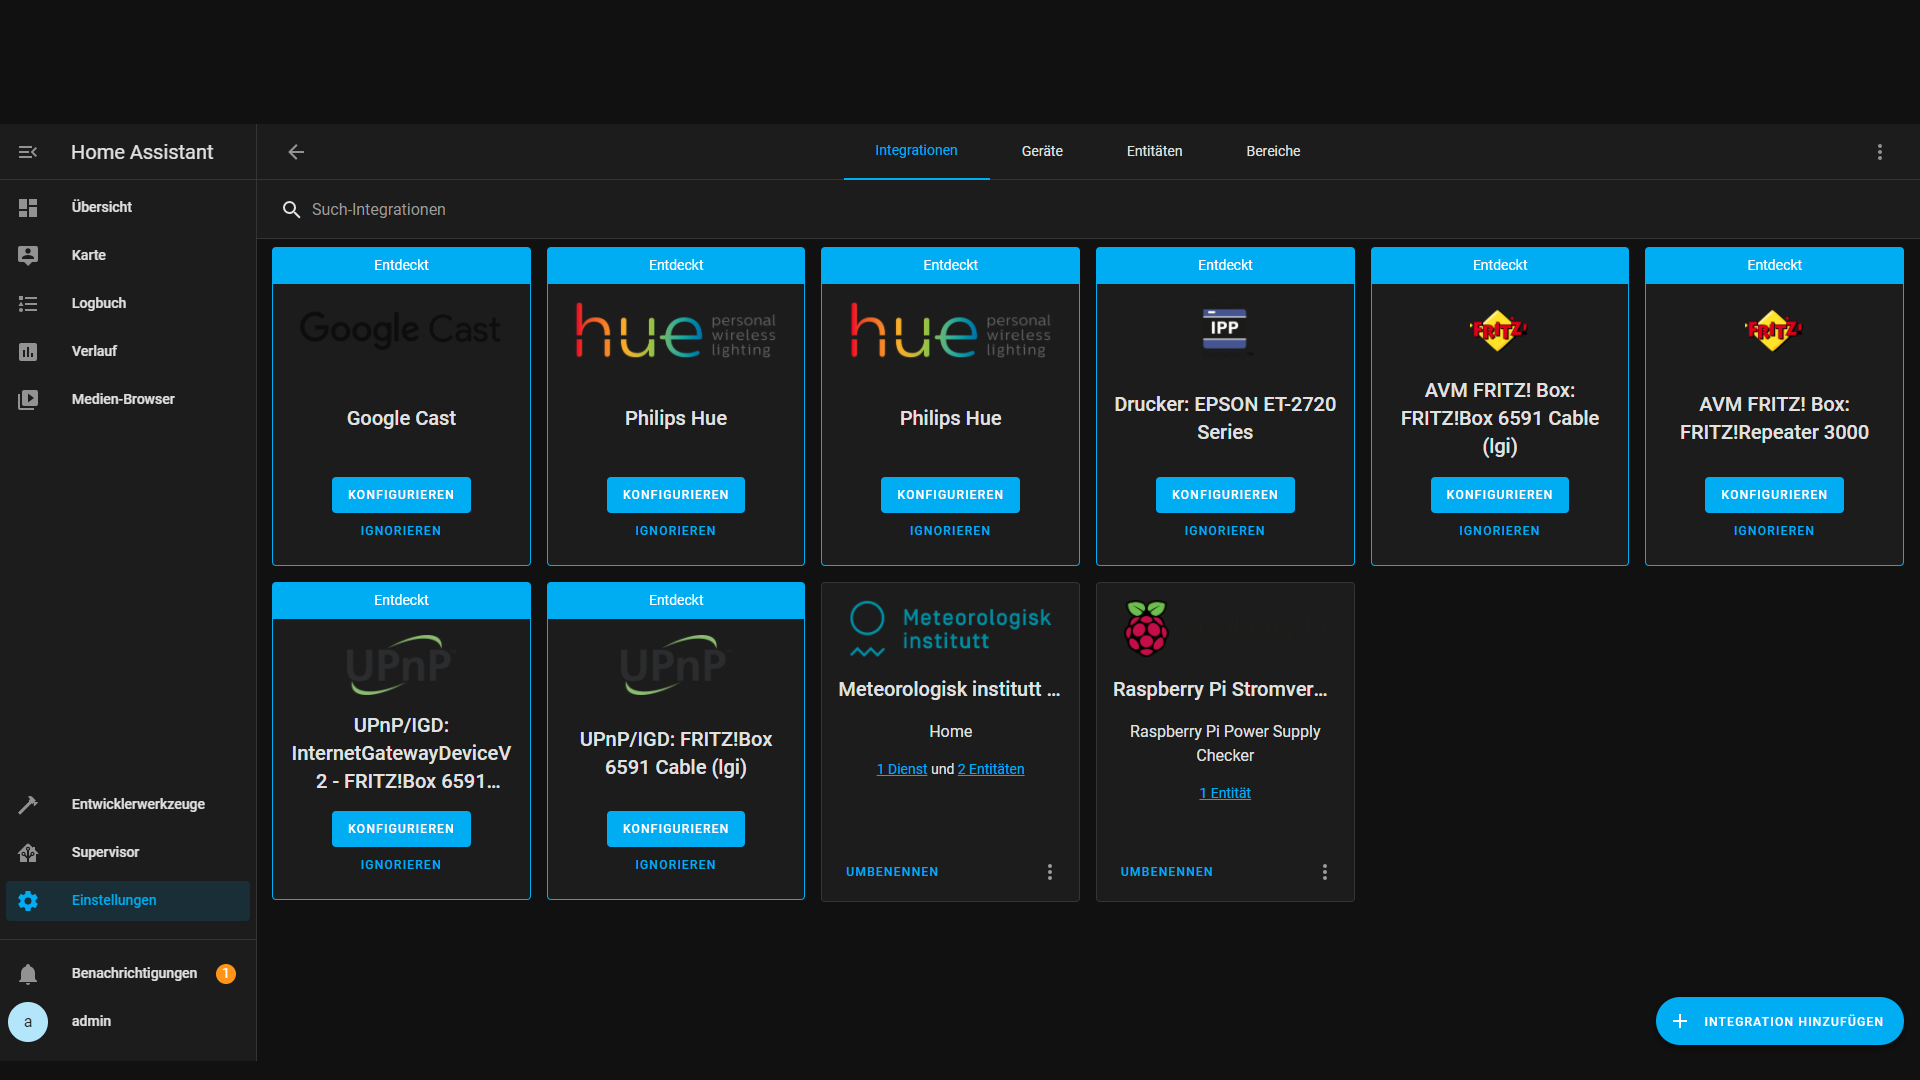
\includegraphics[width=1\textwidth]{img/HA12.png}
        \caption{Startseite Integrationen }
        \label{fig:ha11}
    \end{subfigure}
    \begin{subfigure}{.5\linewidth}
        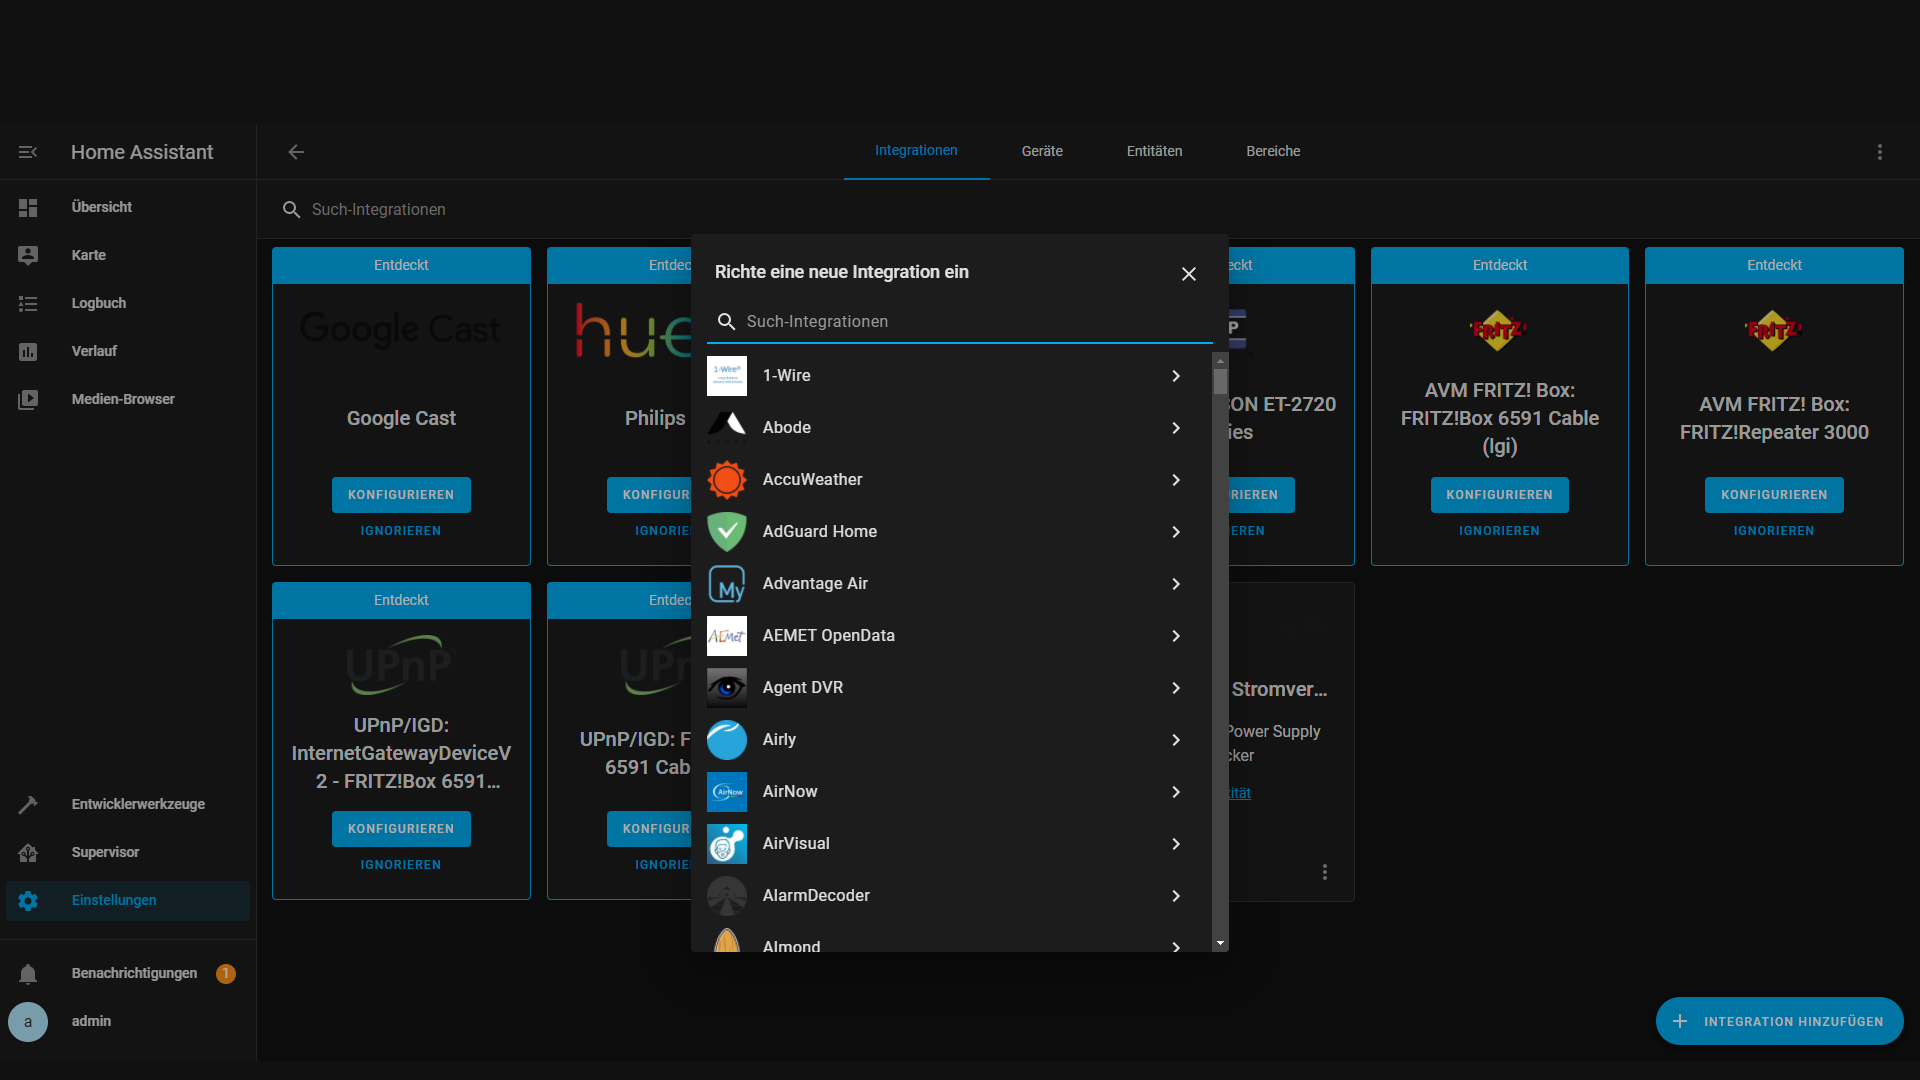
\includegraphics[width=1\textwidth]{img/HA13.png}
        \caption{Suchfunktion Integrationen }
        \label{fig:ha12}
    \end{subfigure}
    \begin{subfigure}{.5\linewidth}
        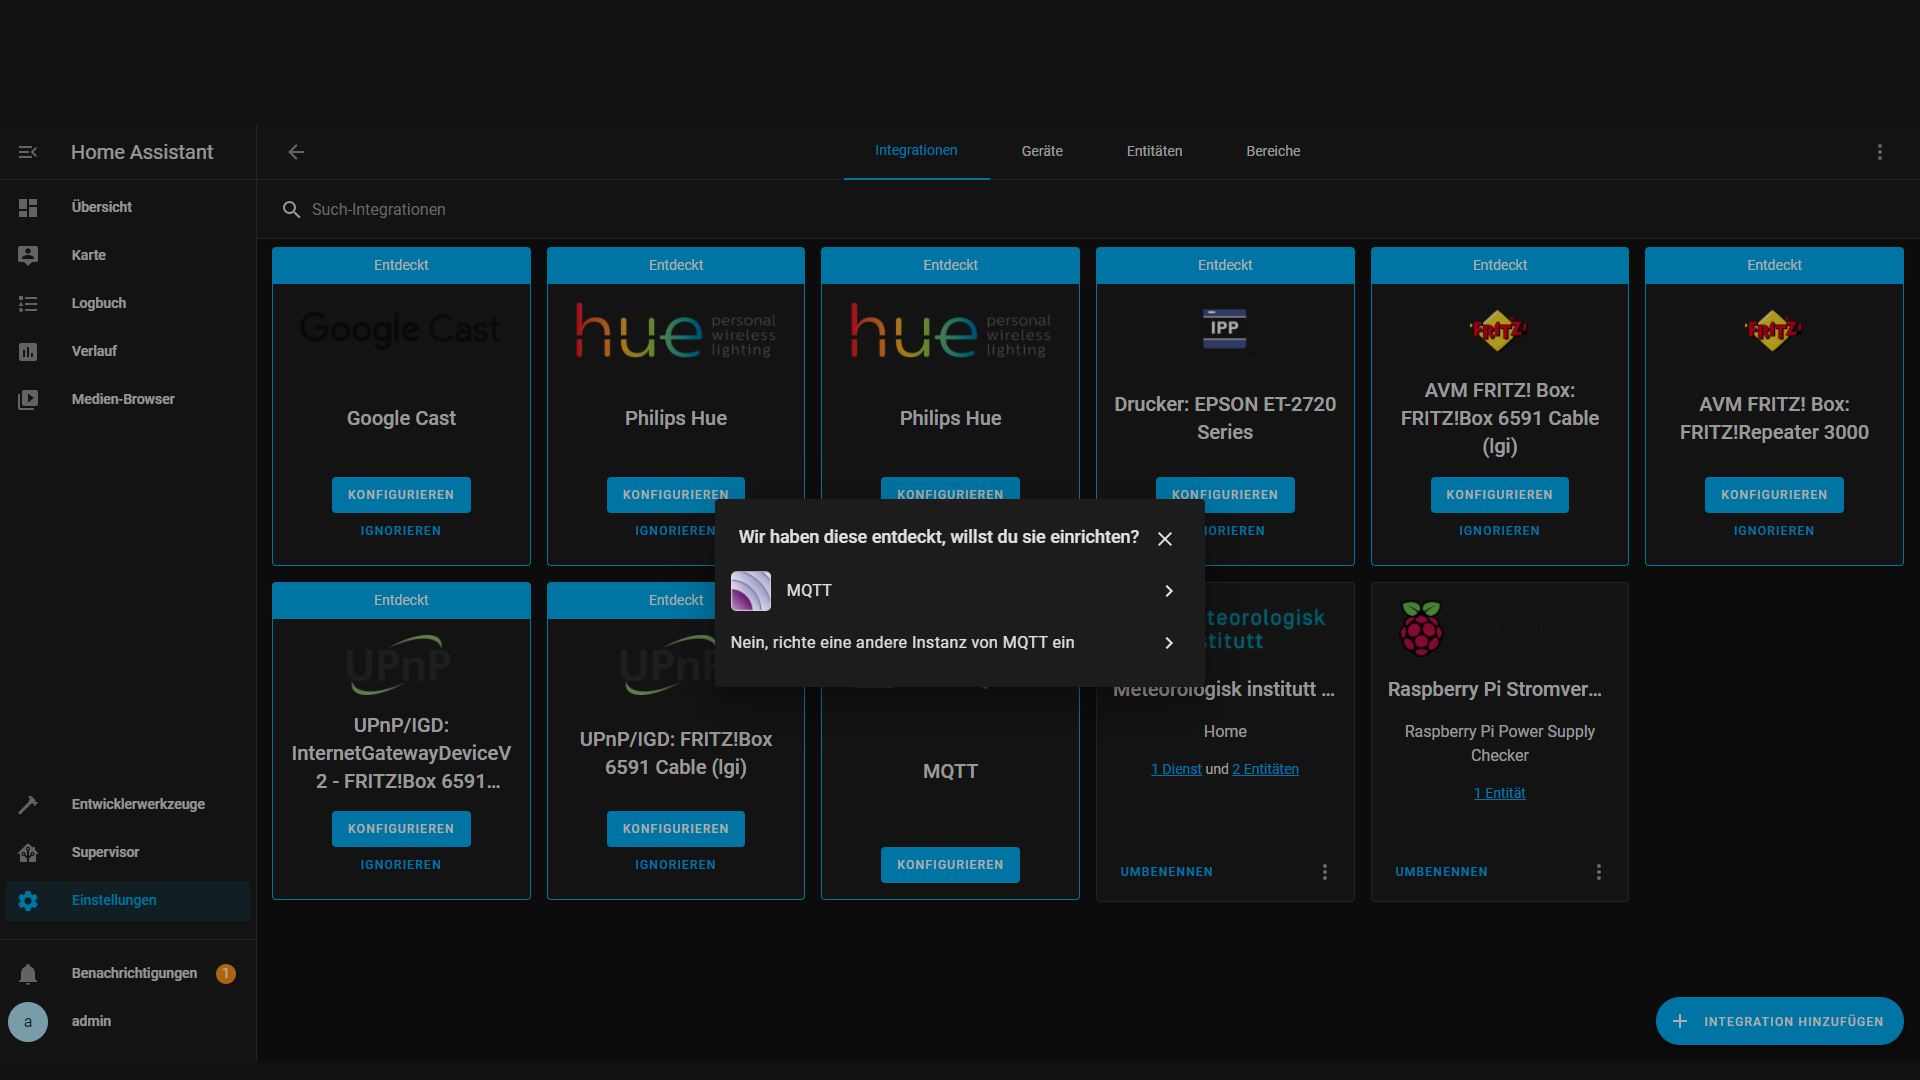
\includegraphics[width=1\textwidth]{img/HA14.png}
        \caption{Suche nach MQTT }
        \label{fig:ha13}
    \end{subfigure}
\end{figure}

%\begin{figure}[H]
%    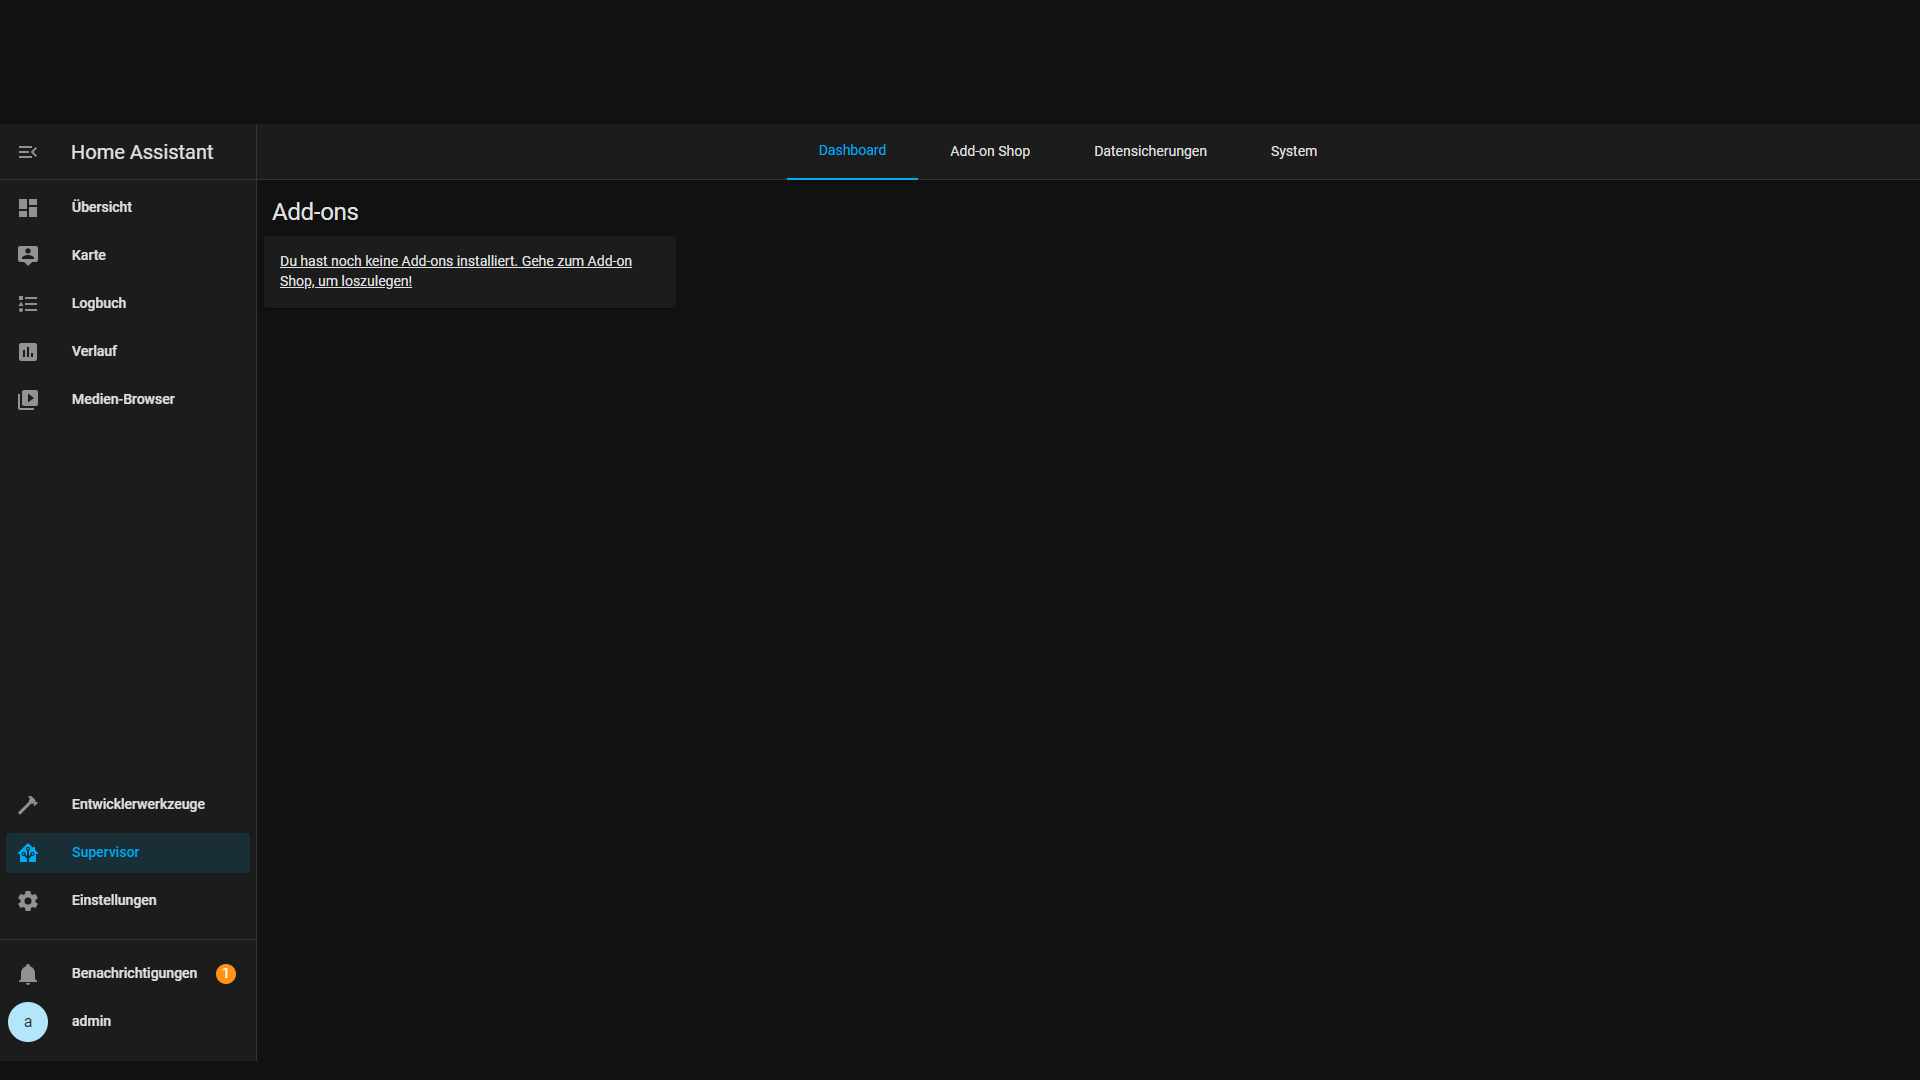
\includegraphics[width=1\textwidth]{img/HA6.png}
%    \caption{Supervisor Dashboard}
%    \label{fig:ha5}
%\end{figure}
%\begin{figure}[H]
%    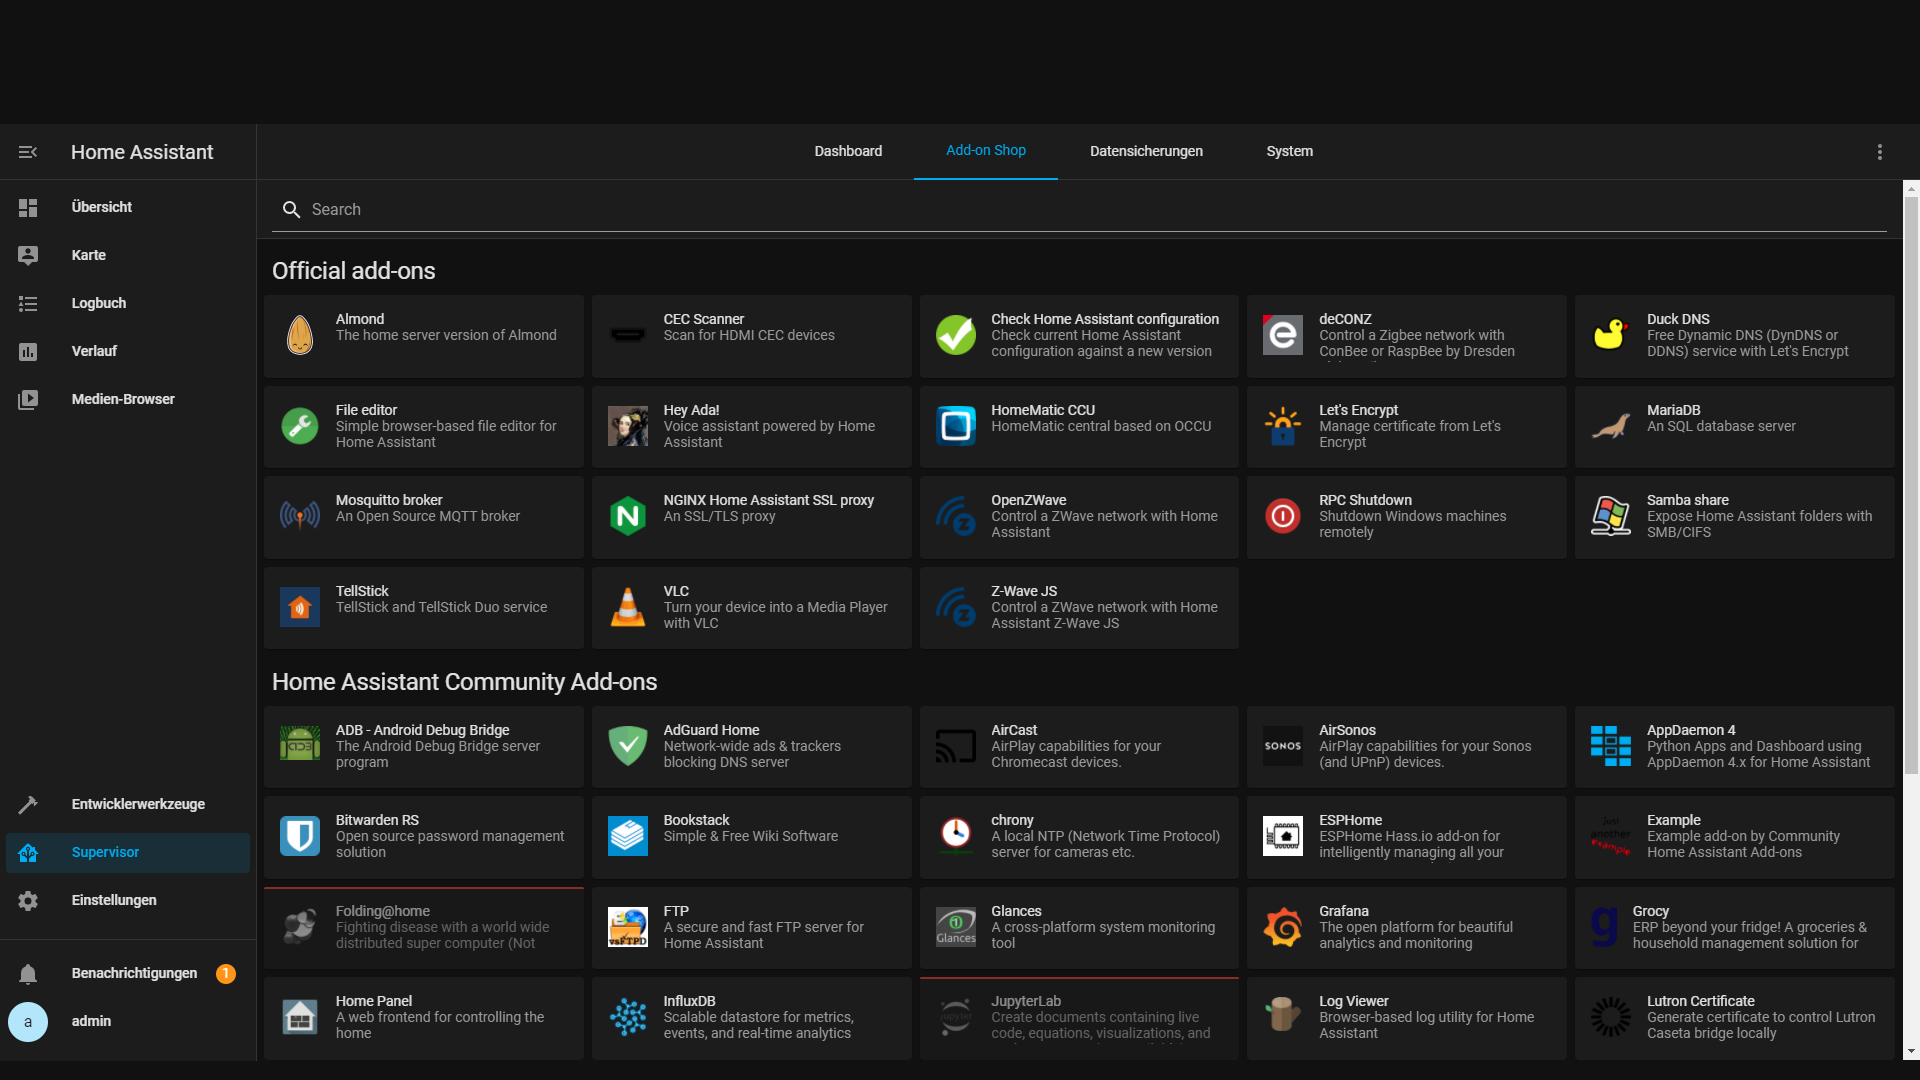
\includegraphics[width=1\textwidth]{img/HA7.png}
%    \caption{Supervisor Add-on Shop}
%    \label{fig:ha6}
%\end{figure}
%\begin{figure}[H]
%    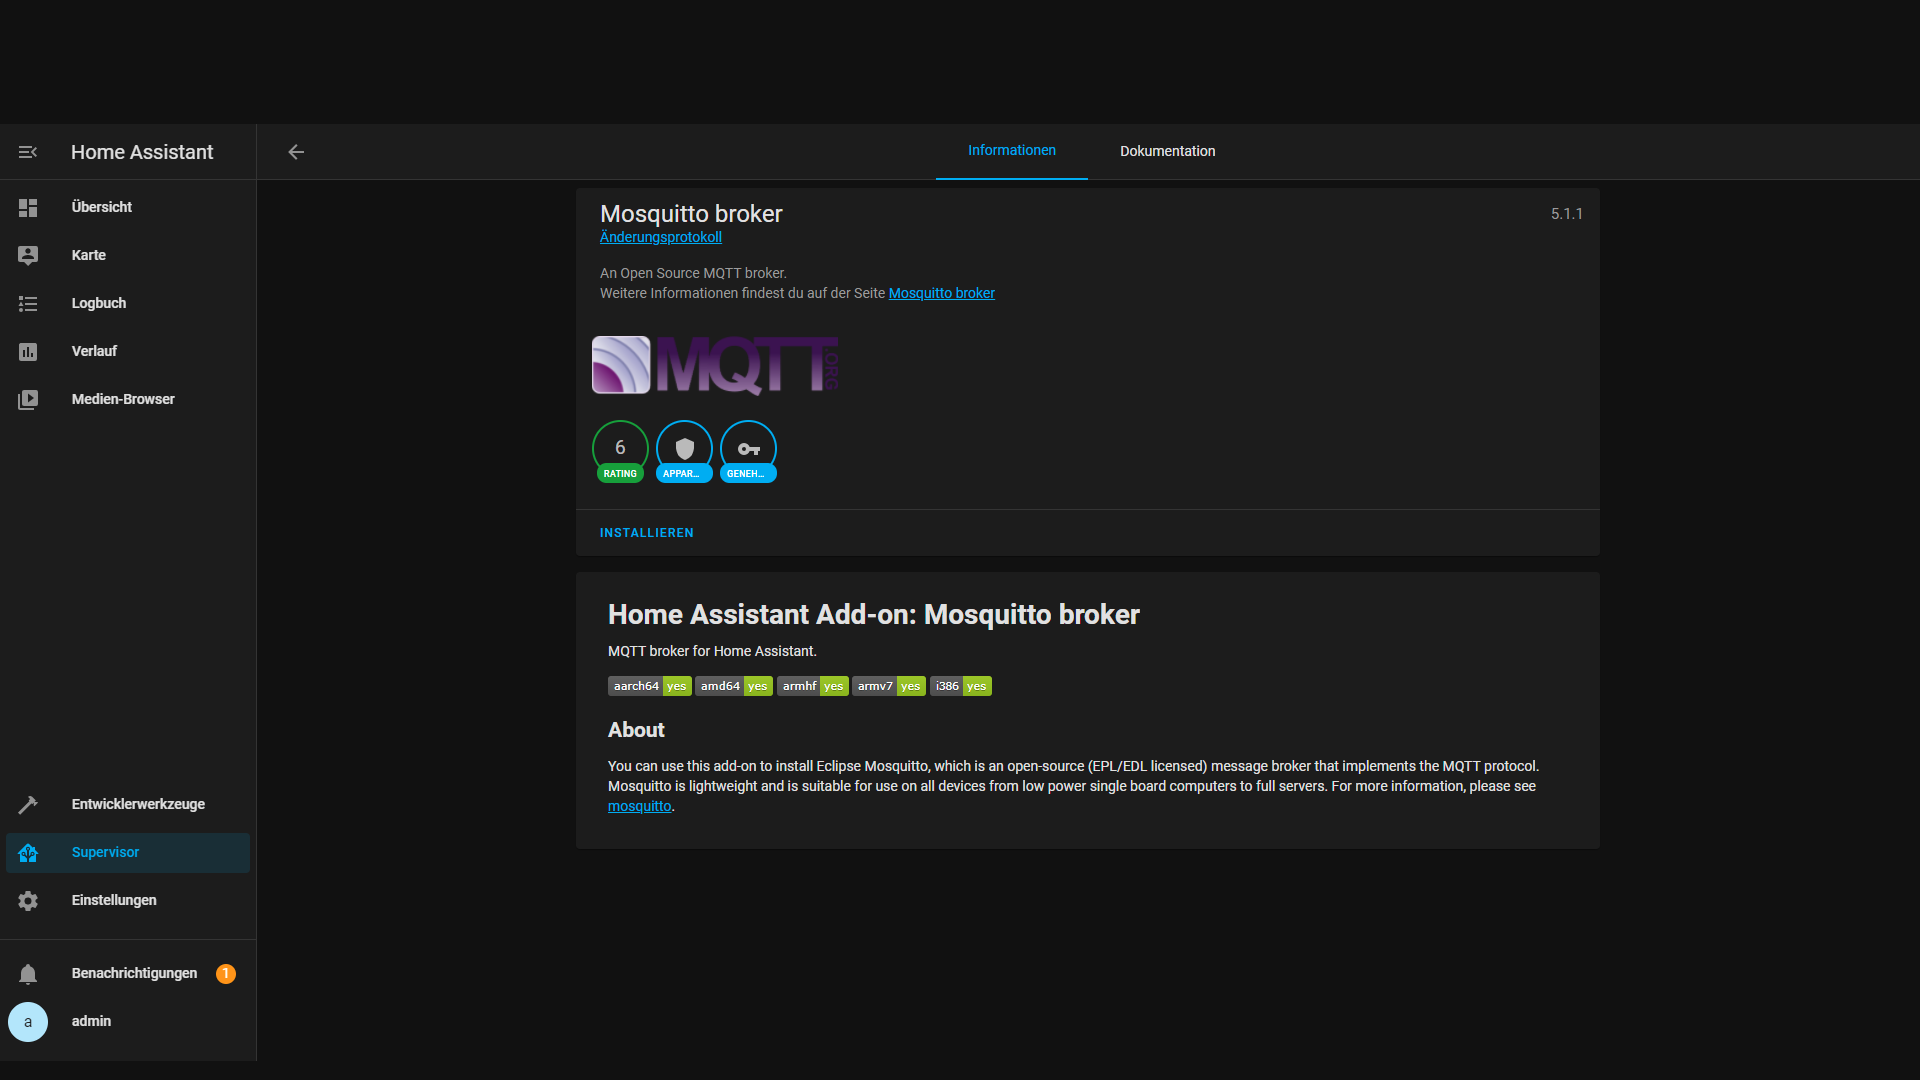
\includegraphics[width=1\textwidth]{img/HA8.png}
%    \caption{MQTT add-on seite }
%    \label{fig:ha7}
%\end{figure}
%\begin{figure}[H]
%    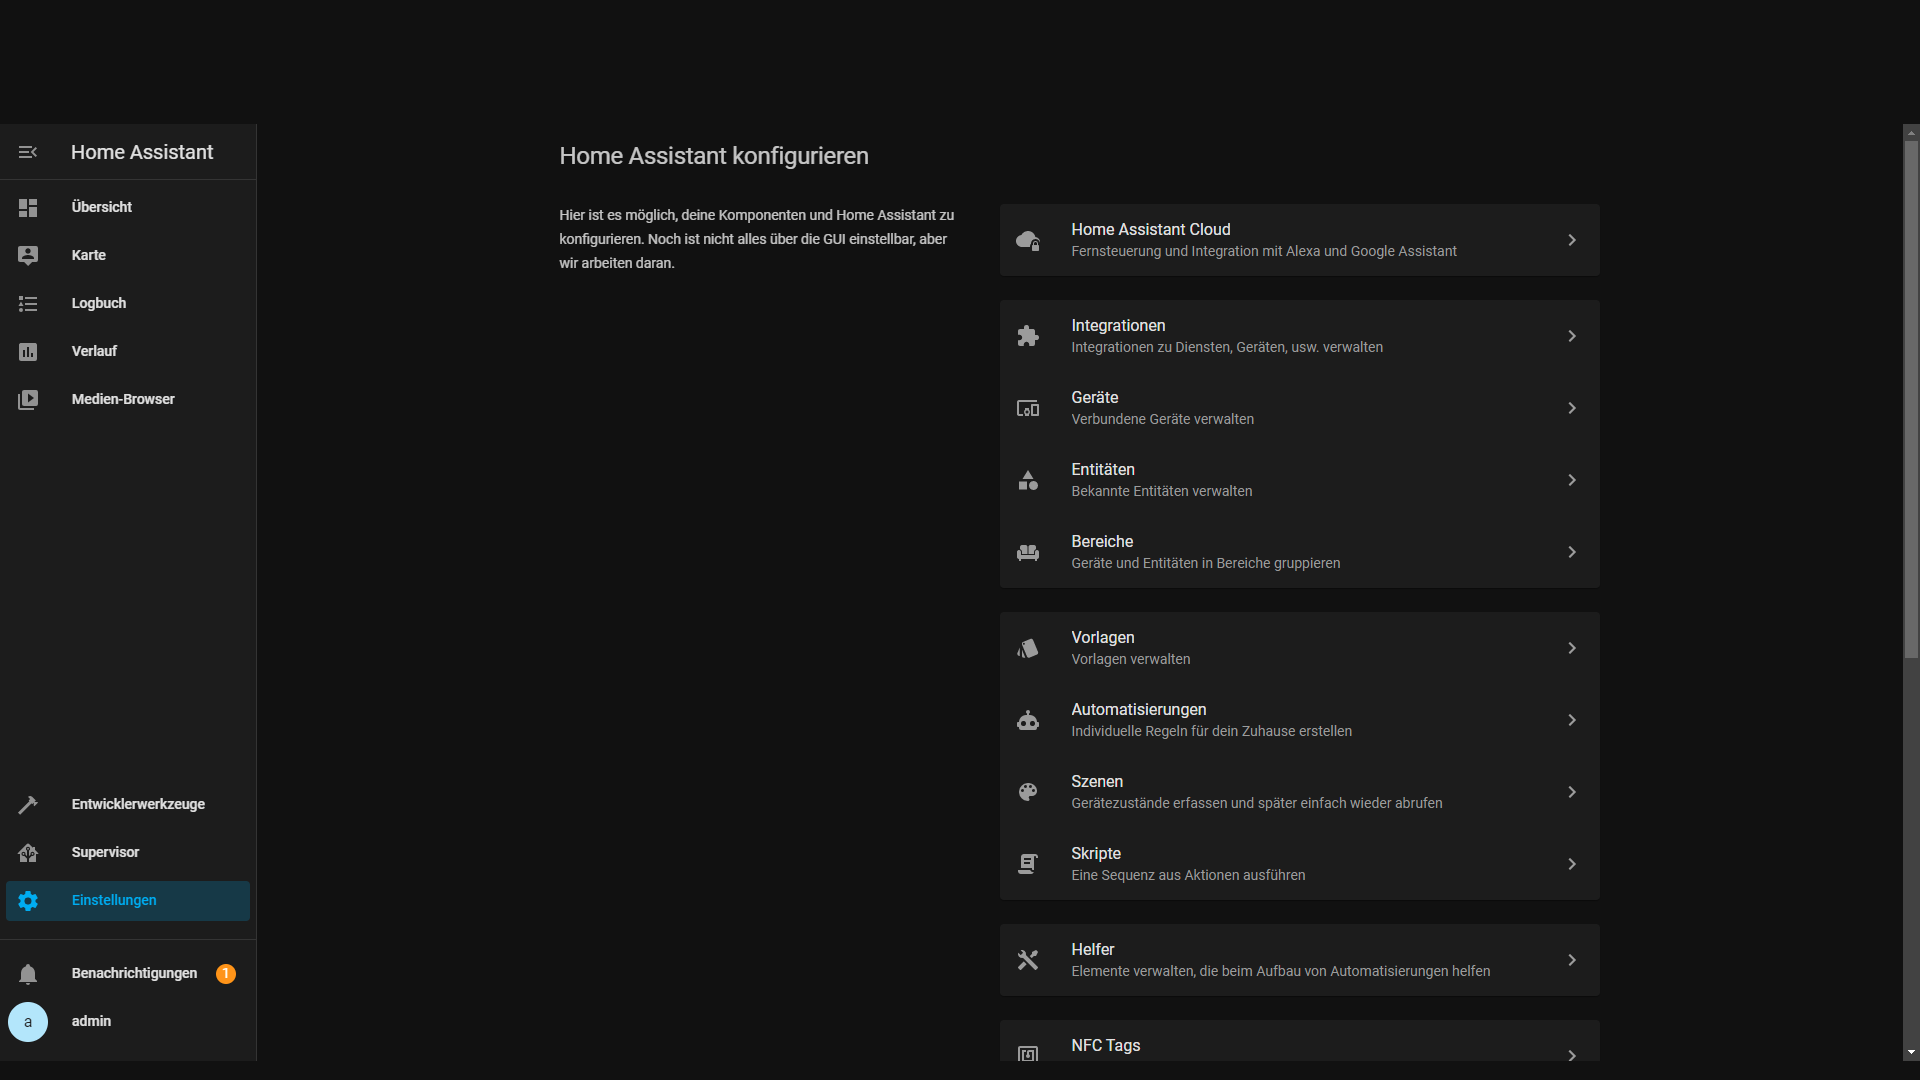
\includegraphics[width=1\textwidth]{img/HA9.png}
%    \caption{Einstellungen}
%    \label{fig:ha8}
%\end{figure}
%\begin{figure}[H]
%    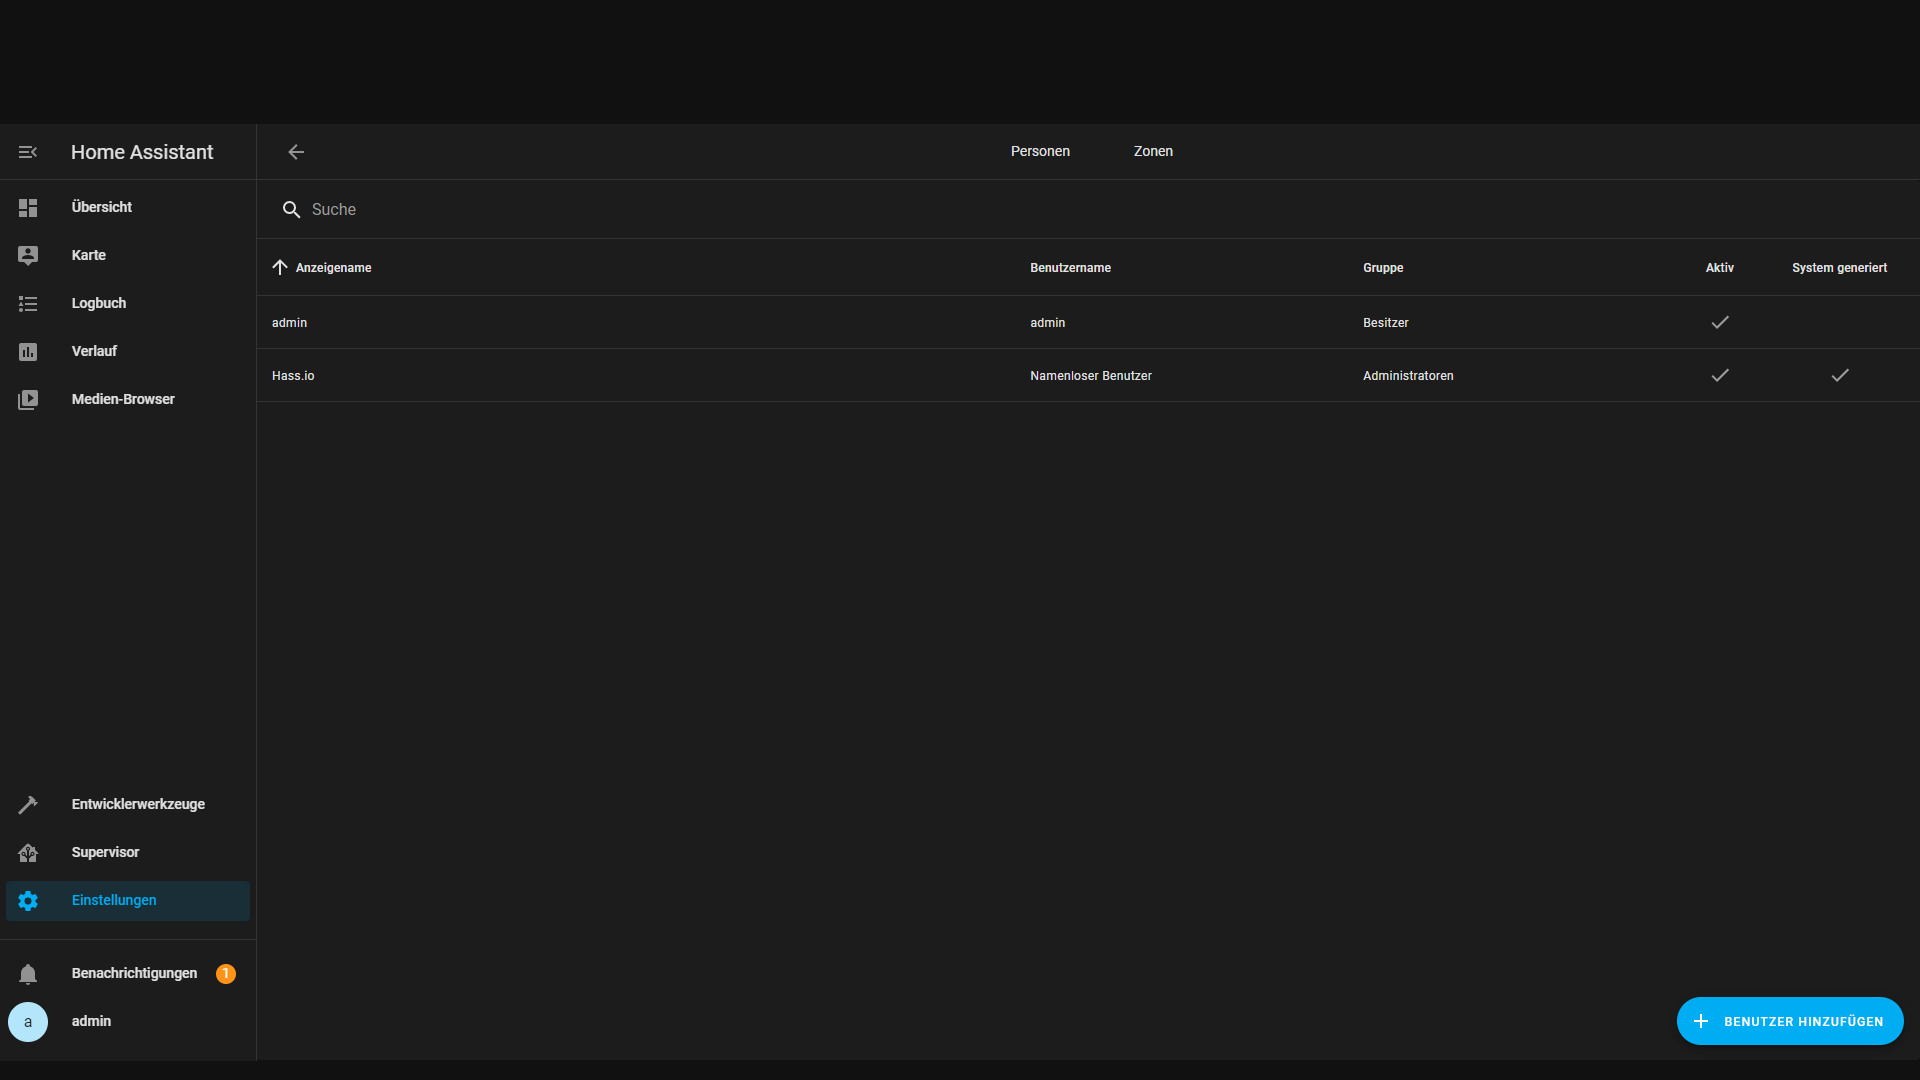
\includegraphics[width=1\textwidth]{img/HA10.png}
%    \caption{Benuterverwaltung}
%    \label{fig:ha9}
%\end{figure}
%\begin{figure}[H]
%    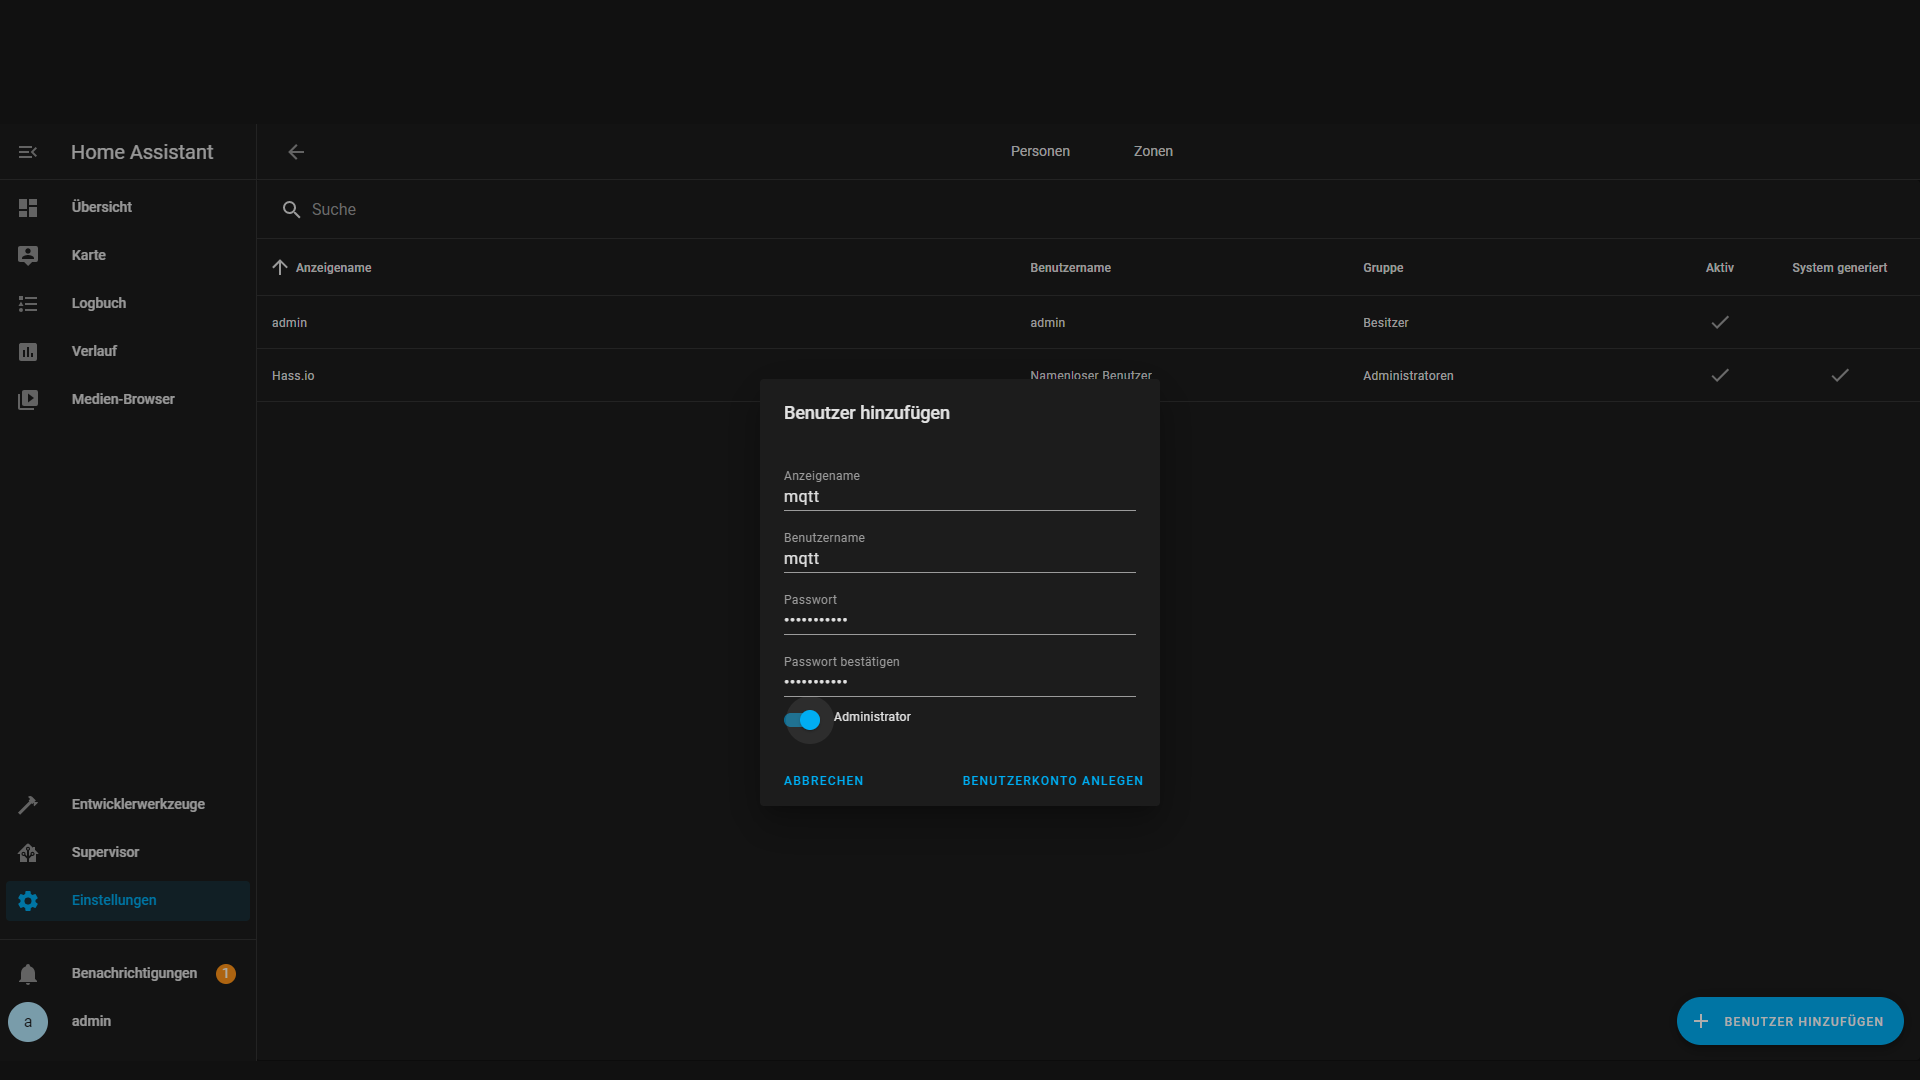
\includegraphics[width=1\textwidth]{img/HA11.png}
%    \caption{Benutzer MQTT anlegen }
%    \label{fig:ha10}
%\end{figure}